\section{Introduction}
\label{introduction}

In the last 10 years GPUs computing has transformed the high performance 
computing, machine learning, and data analytics fields that were previously 
dominated by CPU-based 
installations~\cite{intersect360,cudnn,Lavin15b,SimonyanZ14a}. Many systems now 
rely on a combination of GPUs and CPUs to leverage high throughput data parallel 
GPUs with latency critical execution occurring on the CPUs. In part, 
GPU-accelerated computing has been successful in these domains because of native 
support for data parallel programming languages~\cite{CUDA7,OPENCL} that reduce 
programmer burden when trying to scale programs across ever growing data sets.

\begin{figure}[t]
\centering
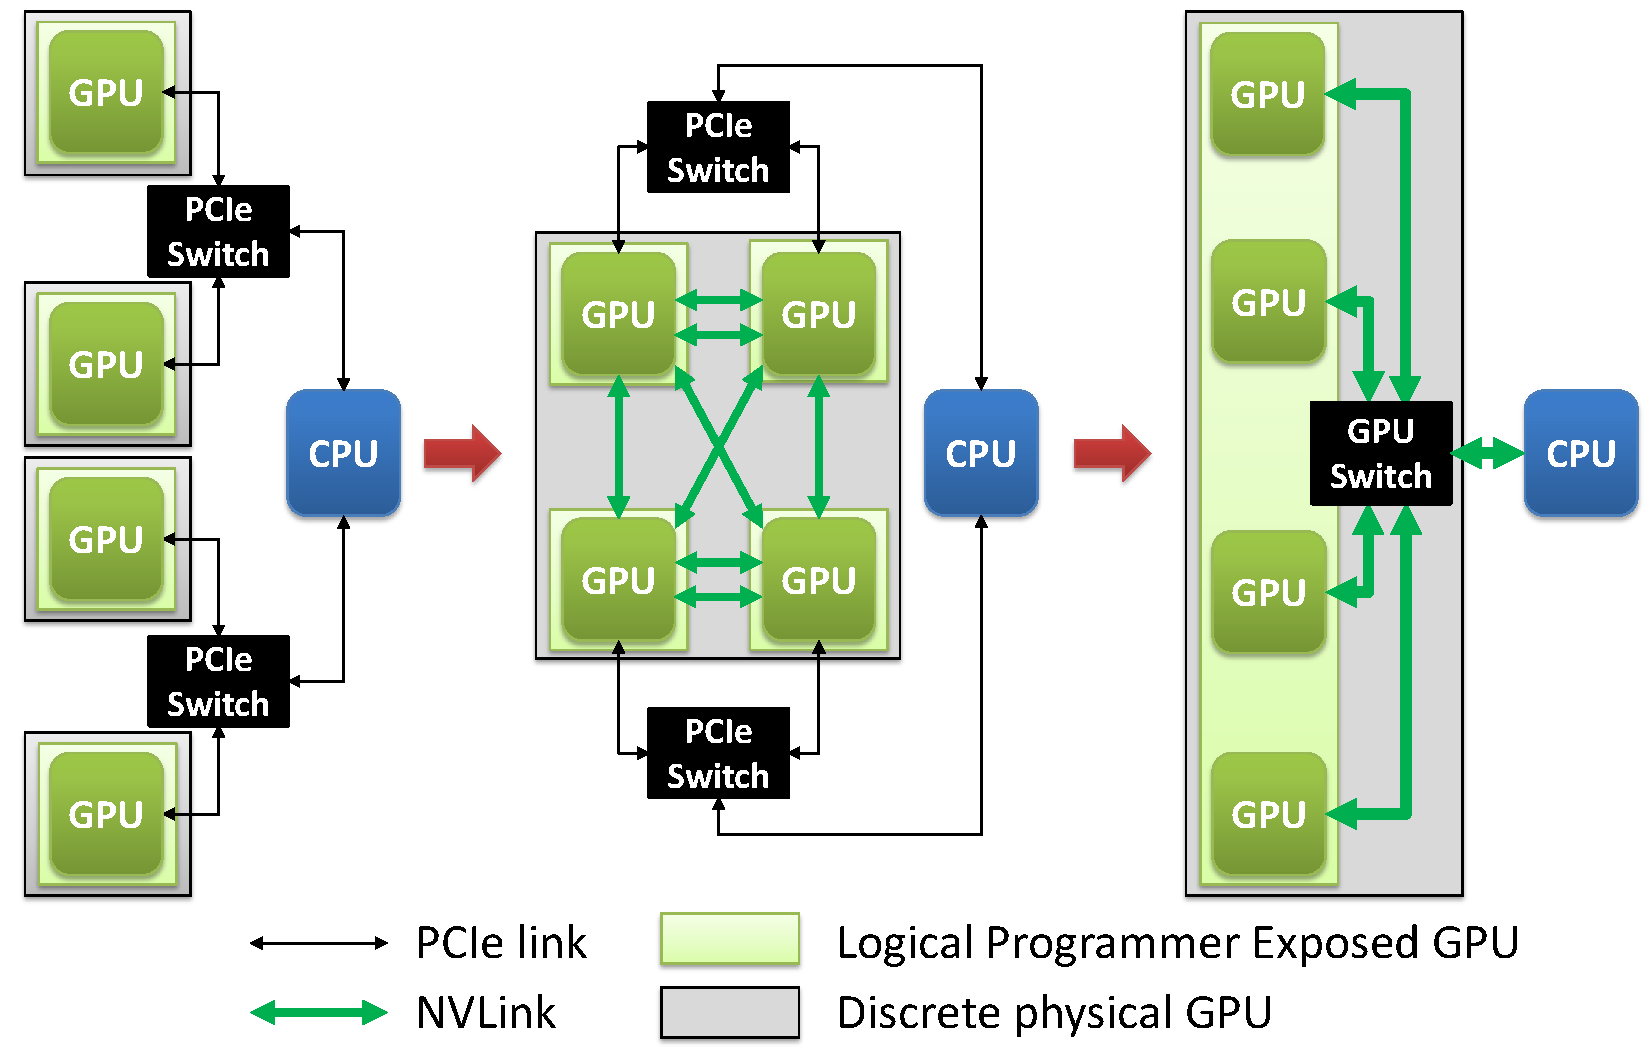
\includegraphics[width=1.0\columnwidth]{figures/inter_gpu_connections.pdf}
\caption{The evolution of GPUs from multiple discrete PCIe devices to 
single logical, multi-socket accelerators utilizing switched interconnects.}
\label{fig:systemdiagram}
\vspace{-.2in}
\end{figure}

Nevertheless, with GPU dies nearing the reticle limitation for maximum die size 
and the transistor density growth rate slowing down~\cite{mooredead2016}, 
developers looking to scale the performance of their single GPU programs are 
in 
a precarious position. Multi-GPU programming models support explicit 
programming 
of two or more GPUs, but it is challenging to leveraging special mechanisms 
such 
as Peer-2-Peer access~\cite{NVIDIAP2P} or a combination of MPI and 
CUDA~\cite{NVIDIAMPI} to manage multiple GPUs. While these programming 
extensions enable advanced programmers to utilize more than one GPU for high 
throughput computation, they require re-writing of traditional single GPU 
application which may slow their adoption rate.

Recently GPUs have started transitioning from using the PCIe peripheral 
interface to having single protocol interconnections between both the GPUs and 
CPUs~\cite{dgx,SierraHPC,AMDINFINITYFABRIC}, as shown in 
Figure~\ref{fig:systemdiagram}. As a result the physical interface of GPUs is 
transitioning away from a discrete pluggable PCIe card into a high pin-count 
socketed processor similar to CPU designs. The socketed interface is required 
not only for power delivery but because the GPU and CPU interconnects require 
printed circuit board (PCB) level integration to provide the needed 
interconnect bandwidth that can be an order of magnitude higher than PCIe 
bandwidths. The evolution of GPUs from externally connected devices to high 
connectivity multi-socket designs is a natural progression as interconnect 
bandwidth becomes a performance critical system component.

The onset of multi-socket GPUs provides a pivot point for GPU and system 
vendors. On one hand, they can continue to expose multi-socket GPUs as 
individual GPUs and force programmers to use multiple programming paradigms to 
leverage multiple GPUs. On the other, vendors may choose to expose multi-socket 
designs as a single non-uniform memory access (NUMA) GPU resource.  By 
extending the single GPU programming model to multi-socket GPUs,  applications 
can scale beyond the bounds of Moore's law, while simultaneously retaining the 
single GPU programming model that GPU developers have become accustomed.

Prior work has examined aggregating multiple GPUs together under a single
programming model~\cite{lee2013transparent,Cabezas2015}, however much of this 
work
was done in an era where GPUs had limited memory addressability
and relied on high latency, low bandwidth PCIe interconnects.
As a result, prior work focused primarily on improving the multi-GPU programming
paradigm rather than achieving highly scalable performance.
However today, in the the era of unified virtual addressing~\cite{UVM},
cache line addressable high bandwidth interconnects~\cite{NVLINK}, and dedicated 
CPU--GPU
socketed PCB designs~\cite{SierraHPC}, scalable multi-GPU performance
may be achievable.

Building upon prior work, we propose a multi-socket NUMA-aware GPU architecture 
and runtime that aggregates multiple-GPUs into a single large GPU and achieves 
good performance scalability across a wide range of benchmarks.  First we apply 
several known NUMA techniques from the CPU community to enable a locality aware 
multi-GPU runtime but show these optimizations are not enough to achieve 
performance scalability in a multi-socket NUMA GPU.  We then propose 
interconnect and cache improvements for GPUs to make their architecture 
~\textit{NUMA-aware} and show that with these improvements multi-socket GPUs can 
achieve good performance scalability when executing programs optimized for a 
legacy single-die GPU. In this work, we make the following contributions:

\begin{itemize}

\item We show that traditional NUMA memory placement and 
scheduling policies are not sufficient for multi-socket GPUs to achieve good 
performance scalability and then demonstrate that intersocket bandwidth will be 
the primary performance limiter in NUMA GPUs.

\item By exploiting program phase behavior we show that intersocket links (and 
thus bandwidth) should be dynamically varied at runtime to maximize link 
utilization. Moreover, we show that dynamic policy must be determined on a per 
GPU basis, as a global policies will fail to capture per GPU phase behavior.

\item We show that both L1 and L2 caches within the GPU must be made NUMA-aware 
and dynamically vary caching policy to minimize multi-socket NUMA effects.  We 
show that the benefit of extending cache coherence across multiple GPU sockets 
far outweighs the overhead of a course grained coherence implementation.

\item Using a NUMA-aware runtime and GPU microarchitecture we demonstrate that
future  multi-socket GPUs may allow traditional GPU programs to scale efficiently to as 
many as 8 GPU sockets, providing significant headroom before programmers must 
re-architect applications to obtain performance scalability.

\end{itemize}
